\chapter{Hardware Implementation}
\label{chapter:3}
% **************************** Define Graphics Path **************************
\ifpdf
    \graphicspath{{Chapter3/Figs/Raster/}{Chapter3/Figs/PDF/}{Chapter3/Figs/}}
\else
    \graphicspath{{Chapter3/Figs/Vector/}{Chapter3/Figs/}}
\fi

%% NO PERSONAL FORMS us,we,I
%% quotes use like : ``text''
%% after point,doublepoints and commas there must be a BLANK SPACE

The following sections show an overview about the hardware implementation of the Invariant Observer Design. 
It starts with a description about the hardware platform on which the observer runs and some details
about the synthesis tools. 
At the end of this chapter, there comes a design view about the synthesized hardware and a discussion about 
the design steps. 
\section{Hardware Platform for a Prototype}
\label{chapter:3:section:1}
The Invariant Observer is synthesized on a Field Programmable Gate Array(FPGA), on this platform it is possible to get an insight
about the runtime behaviour and to see the observer in action. 
The FPGA board, that was used for the simulations, is a \textbf{DE2-115} modell from ALTERA\cite{altera1}. 
That board is ideal to illustrate fundamental concepts and advanced designs, and it gives a possibility
to meet necessary real-time requirements. The DE2-115 is equipped with a \textbf{Cyclone IV EP4CE115F29} 
FPGA Chip and it is powerful enough to emulate a CPU(ex. Nios from Altera). In \cite{RTFMBJ13} this FPGA board was used for performance studies, besides other FPGA's,
so it was logical to use a similar environment. 
The \textbf{DE2-115} has an on-board oscillator of 50 Mhz and in combination with a Phase Locked Loop(PLL) it is possible to increase the operating frequency for advanced tests. 
In the following section it will be shown, how enhanced frequencies can change the design on the Register Transfer level(RTL) and why bad design decisions 
can influence the maximal speed of a design. In Appendix~\ref{appendix:4} there is a schema illustration about the components of the \textbf{DE2-115} FPGA board. 


\section{Synthesis and Design}
\label{chapter:3:section:2}
This section gives an overview about the synthesis tool and details about the Register Transfer Level design view. 
An interesting part in this section is to see how the synthesis tool creates hardware structures based on the code of the
Observer VHDL implementation. \newline
For synthesis and compilation of the observer VHDL code, the \textbf{Altera Quartus II Version 12.1 Build 177 Full Version} was used. 
\subsection{Design View of the Register Transfer Level}
\label{chapter:3:section:2:sub:1}
In Quartus II, after compilation of the design and after creation of the netlists, you can use a tool named \textbf{RTL Viewer}, which shows how
the components of the design will be created on a Hardware Platform. It is an abstract view on the \textbf{Register Transfer Level}. 
This tool can be very handy if someone want to see how the hardware should look like. Based on the illustration of the hardware, some decisions can
be reconsidered in terms of the performance. \newline
Figure~\ref{fig:test:only:50:obs0} is the hardware schematic view of a single observer stage (m=1), which is modelled as a single observer with input frequency of 50Mhz. 
In which way, this test cases was modelled, will be discussed in the next chapter. 
The next Figure~\ref{fig:test:only:150:obs0} shows exact the same design case like Figure~\ref{fig:test:only:50:obs0} but with the difference that the operating frequency is 150Mhz. 
In Figure~\ref{fig:test:only:150:obs0}, it is illustrated how the syntheses tool reorientates the hardware design, 
to meet the requirements of that clock speed. The worst case path determines the maximum frequency, which is allowed for that design. 
A more detailed description about the timing model is in the next subsection. 
\subsection{Timing Model of the Design}
\label{chapter:3:section:sub:2}
One important thing that have to be considered is that the signal path from the beginning of the observer entity to the end should be as short as possible,  
this concludes to some important design facts.
The maximum frequency of the whole system is limited by the longest path of the design, which means that the performance of a system is expressed by the maximum frequency at which it may be operated. 
So it should be logical for every entity in the netlist, to keep the signal path as short as possible. 
The performance maximum can be computed by the Quartus Tool named \textbf{TimeQuest Timing Analyzer}, which gives estimations about the maximum frequency of the design. 
The longest signal path of a design is indicated by the \textbf{worst case path} in the tool. \newline
The first version of the observer stage had a low performance level, a illustration of this version is shown in the Appendix~\ref{fig:version:one:obs}. 
The TimeQuest Timing Analyzer consider some uncertainties for the performance estimations. From \cite{altera2} it is known how the Quartus Tool creates timing models. These are
created in the TimeQuest Timing Analyzer after building the netlist, as part of the compilation process of a design. 
A FPGA has to operate in a continuum of conditions. These conditions include the die junction temperature which can vary among specific ranges, for example 
commercial parts have a range of 0°C to 85°C and industrials a bigger range. 
A further condition is the voltage supply level with regard to critical voltages for maintaining FPGA performance(Vcc and the various I/O supplies). 
\newline
The timing analyzer shows estimations for three cases
\begin{enumerate}
\item Slow 1200mv 85°C model
\item Slow 1200mv 0°C model
\item Fast 1200mv 0°C model
\end{enumerate}

These are operating-condition corners which are usually end point combinations of the ranges in temperature, voltage and manufacturing processes. 
Each operating-condition is used to model the timing delays under specific end points of temperature, voltage, and manufacturing process conditions. 
The first case with ``Slow 1200mv 85°C model'' seems natural and was more considered for test cases, because it shows frequencies under long term 
operating conditions. 
A lot of tests about estimations of the maximum frequency of different design cases have been exercised(shown in the next chapter), and only the estimations
from ``Slow 1200mv 85°C model'' were significant for further discussions. In the next chapter there is a summary of these tests. 

\subsection{Design Decisions based on Register Transfer level}
\label{chapter:3:section:sub:3}
At the first time, where the VHDL Code of the observer stage was behavioural correct, some performance and optimization decisions had to be reconsidered. 
The most important thing is to separate synchronous and asynchronous design. So, it was necessary to split the first version of a completely synchronous design, where
every action is only triggered after every clock cycle. A more parallel approach was necessary where only state changes are done synchronously, but other actions should
be triggered immediately after any change of the state. And a asynchronous system part can be separated in several independent asynchronous components, which achieves more 
system parallelism and a better performance. As already mentioned in  chapter 2, this system design is similar to a Moore State Machine, where the logic 
is separated in a transition logic, an output logic and a state memory. And only the state memory should be changed on every clock cycle.
The design approach of the invariant observer is similar, but with the difference that the output logic and transition logic components are merged together. 
The hardware schemas from the Register Transfer Level illustrations were beneficial, because they showed how the components where created with its VHDL background. 
For example If-statements should be created in a way, that allow no Latches. This means that every else-branch should contain the same components like the if-branch. 
Following that rule, mutexes will be created which are shown here in the example of Figure~\ref{fig:test:only:50:obs0}. Every mutex has two inputs(according to if, else), which are
selected depending on the third input(MUX21).
At the beginning of the entity there are several adders and these are representations for the different addition operations
which has to be done according to the behaviour of the observer. \textbf{Add2} emulates ``$cycle\_next=cycle+1$'', \textbf{Add1} emulates ``$cycle\_next=cycle-1$'' and \textbf{Add3}
emulates ``$count\_p=count\_p+1$'' according to the sourcecode of the Observer Stages in Appendix~\ref{appendix:source:2}. 
In Figure~\ref{fig:test:only:50:obs0}, the MUX 21 Mutex at the beginning, indicated by \textbf{cycle\_next[15..0]}, is the if-branch, according to the sourcecode in Appendix~\ref{appendix:source:2}, 
which decides if ``$cycle=0$'' or not.
The \textbf{MUX21[cycle\_next[31..16]]} below stands for the branch ``if $cycle=observernumber$''. 
\textbf{MUX21[cycle\_next[15..0]]} decrements cycle\_next in normal case, but increments it only once if the value of cycle\_next reaches the bottom limit. 
\textbf{MUX21[cycle\_next[31..16]]} works the opposite way. 
As you can see, the tool enhanced cycle\_next up to 48bit to reserve memory for intermediate results.
In the middle of the hardware scheme, there are two another \textbf{MUX21[cycle\_next[15..0]]}, 
the first(left to right) decides between  ``$cycle\_next=cycle+1$'' or ``$cycle\_next=cycle-1$'' and the second 
between the result from first Mutex before and the reset value. \textbf{MUX21[cycle\_next[47..32]]} decides between keeping the old value ``$cycle\_next=cycle$'' or 
taking over the value from \textbf{MUX21[cycle\_next[31..16]]}. The overview regarding count\_p is similar, but a deeper insight about that Quartus translation behaviour would exceed that subsection. 
As you can see in the hardware schema, there are 5 registers(cycle, count\_p, direction, output, enable\_out) 
and these representates the state of the Invariant Observer and they may only change their values after every clock\_cycle. 
The dimensions of the registers are conform to the dimensions of the input conditions. 
For example if inc\_tau has a value with only 5 bits, then count\_p is accordingly large-dimensioned to 6 Bit. 
This is only a cut-out, about how the Quartus II translates VHDL Code. 
A lot of other hardware representations are shown in Appendix~\ref{appendix:3}, actually they have the same components but another orientations. 
The next subsection shows something about problems during the progress of that development. 

\begin{figure}[]
\centering
%\hspace{3.0cm}
%\vspace{-5cm}
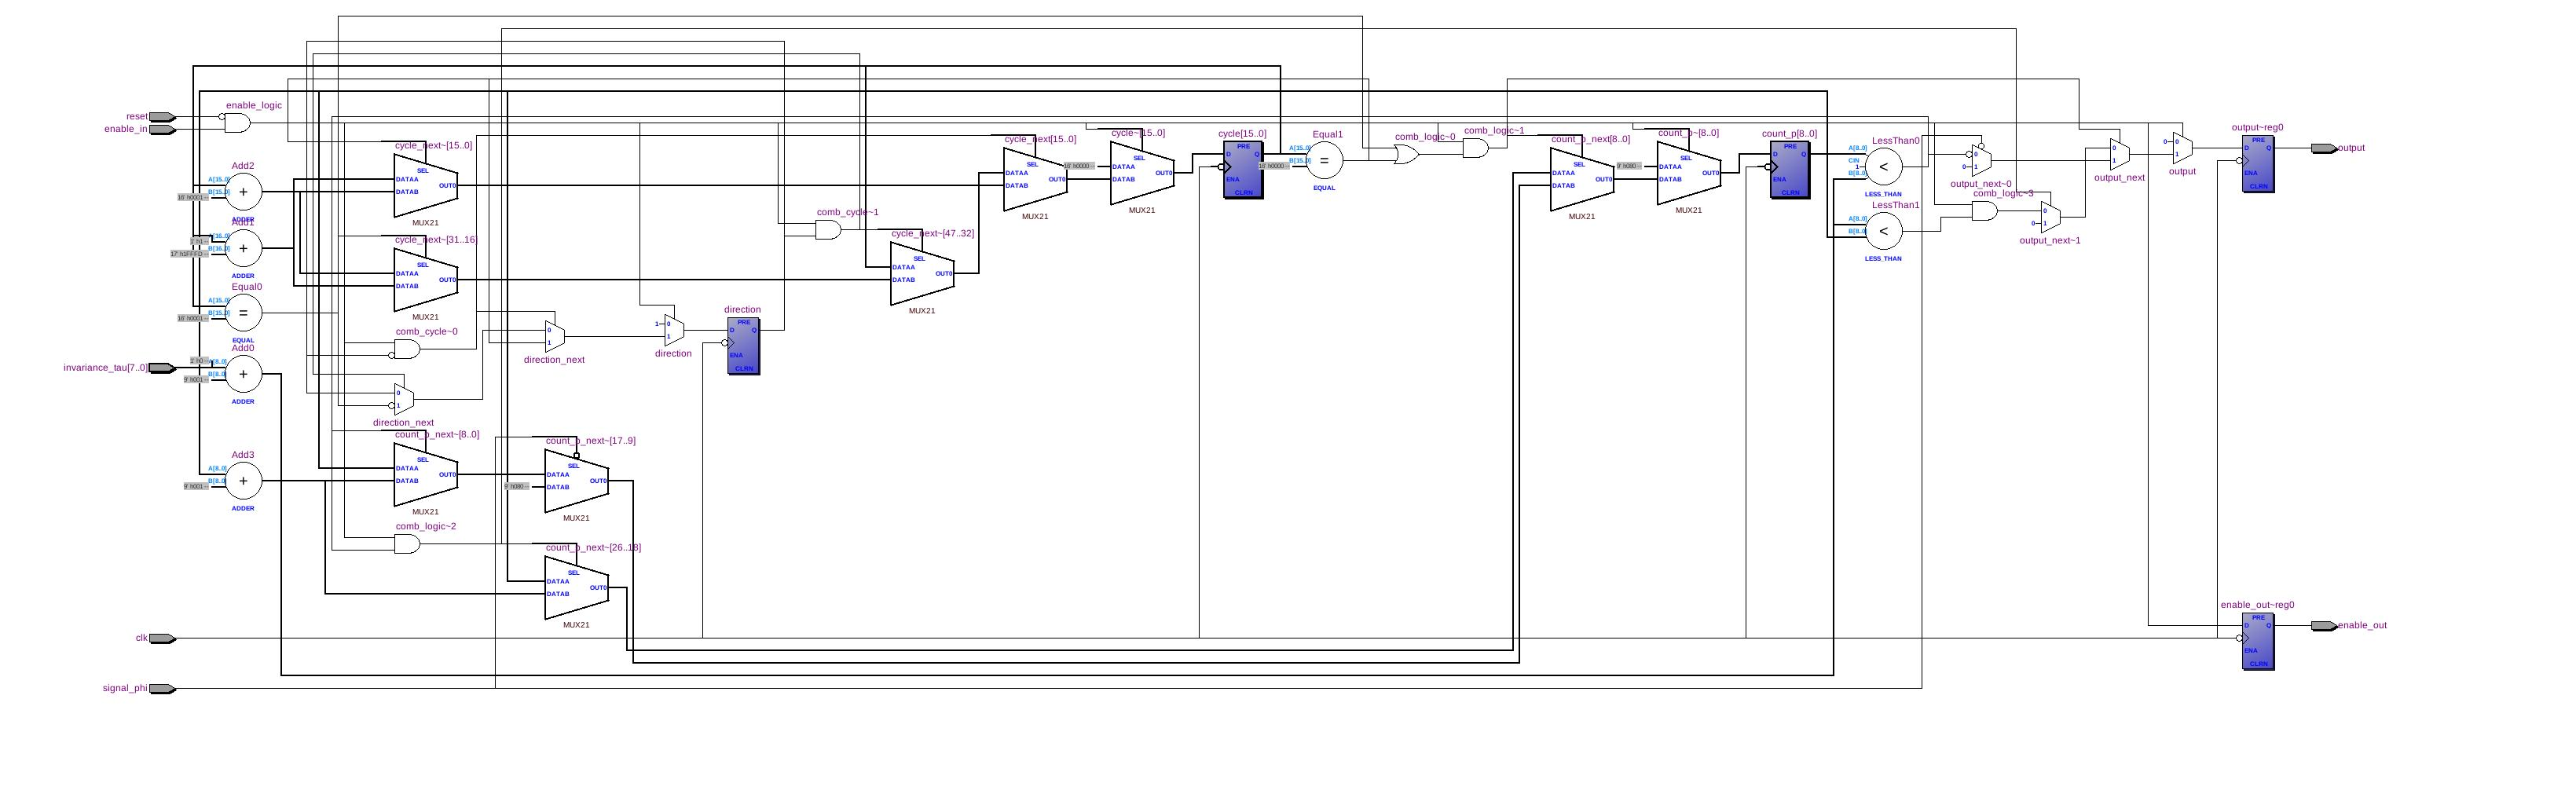
\includegraphics[width=650px,height=300px,angle=-90]{../../pictures/22.02.2014/onlyObserver/OBS_50M.jpg}
\caption[RTL View of Observer 0 with clock 50Mhz]{Shows a RTL View of a single observer stage with input clock of 50Mhz}
\label{fig:test:only:50:obs0}
\end{figure}

\begin{figure}[]
\centering
%\hspace{3.0cm}
%\vspace{-5cm}
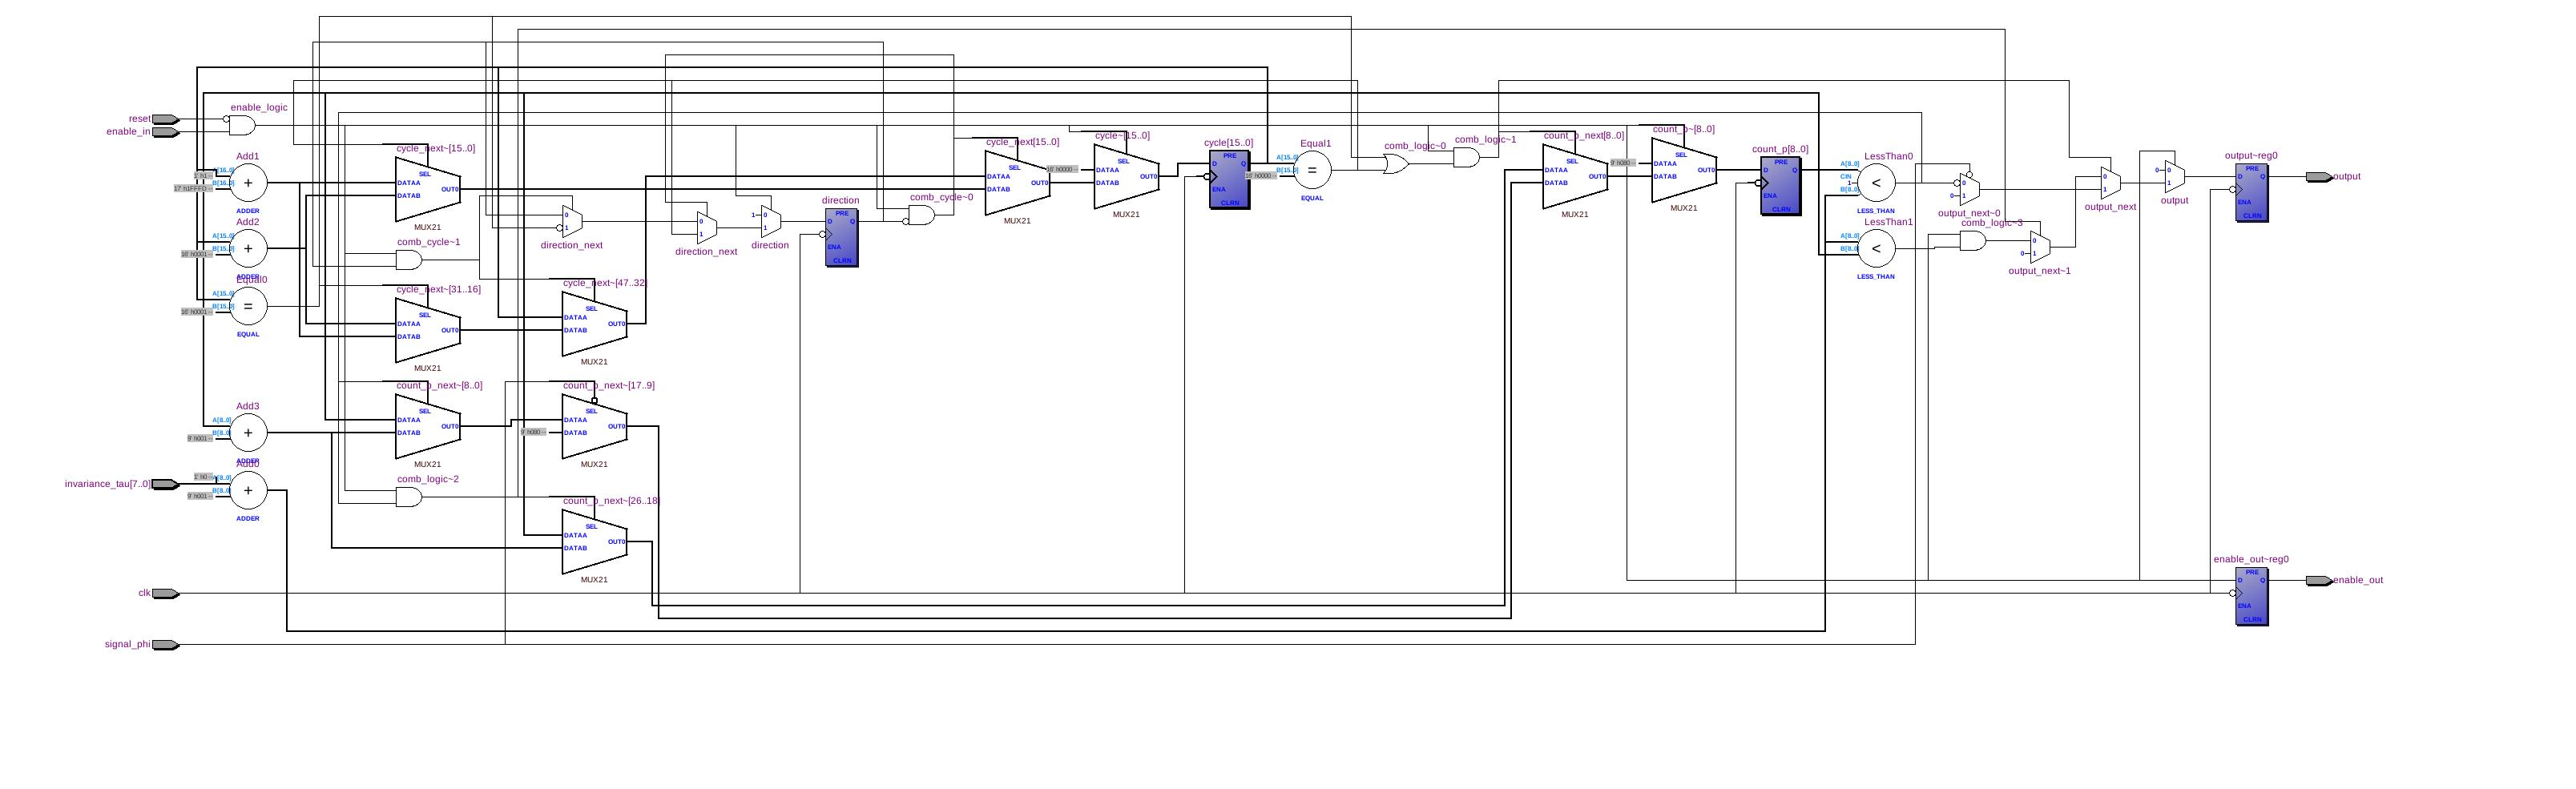
\includegraphics[width=650px,height=300px,angle=-90]{../../pictures/22.02.2014/onlyObserver/OBS_150M.jpg}
\caption[RTL View of Observer 0 with clock 150Mhz]{Shows a RTL View of a single observer stage with input clock of 150Mhz}
\label{fig:test:only:150:obs0}
\end{figure}

\newpage
\section{Design problems in the development}
\label{chapter:3:section:3}
This subsection is only a kind of a protocoll about problems during the development. 
\begin{enumerate}
\item The starting condition of the Algorithm~\ref{alg:observerstage} was uncertain, the question was, should variable
count be initialised with 0 or with ($\tau + 1$). If count=($\tau + 1$) then the output is immediately switched on, which
correspond to an invariance qualification. From the specification of an observer in \cite{RTFMBJ13}, it is known from
the proof of Theorem 1(in \cite{RTFMBJ13}) that $\forall i:(i \in [max(0,n-\tau),n] \rightarrow e^i \models \phi)$ which follows 
that at the beginning of an execution if $n-\tau$ exceeds th bottom border, but the signal $\phi$ is true, the invariance qualification
is fulfilled by that specification. 
This condition only holds if signal $\phi$ is known at that time, in our case the status of signal $\phi$ is always(if $m \ge 1$) taken from the past. 
So it is not known which status the signal $\phi$ has before execution time $e^0$. Hence, the Algorithm~\ref{alg:observerstage} was initialised in a manner, that
no decisions can be made about invariance qualifications. 
\item The Invariance Observer was tested with a  self-made signalgenerator which imitates input $\phi$. As a result, two clock domains were created, although the clock signals
came from the same PLL(Phase Locked Loop). If the observers clock is an "even" multiple of the second clock frequency(signalgenerator), there was no problem, but if the clock frequencies are choosed in a different way, then
it comes to clock drifts. 
\item The file (*.sdc file)for timings has to be adjusted every time, if there are changes in one of the clock domains. The PLL output timings have to be analyzed separately by the
TimeQuest Timing Analyzer. If this does not happen, false estimations are created for "Slow 1200mv 85°C model" maximum frequencies and worst case paths. 
\item The first download of the compiled design to the FPGA was no succesfull, because the Quartus Tool was not correctly adjusted to that plattfom. 
Following points had to be changed:
\begin{itemize}
\item The correct architecture must be set
\item the voltage level must be set for all inputs and outputs
\end{itemize}
\item It should be always considered what is the active state of an input component or output component, for example
input KEY is low active and it was used to reset the FPGA board. 
\end{enumerate} 
